\section{Aspectos del Negocio} \label{sect:aspectos_negocio}
  
Al consistir el proyecto de pasantía en el desarrollo de la versión móvil para el portal \textit{Tuguia.de}, se hace necesario comprender algunos de los conceptos y términos asociados con el negocio y de esta manera facilitar el entendimiento de los posteriores capítulos.

\subsection{Contenido del Sitio} \label{subsect:contenido}

El contenido de \textit{Tuguia.de} es bastante variado, si bien el sitio esta planteado como una guía de locales, el portal no solo ofrece información sobre estos, también cuenta con contenido que corresponde a otro tipo de establecimientos y servicios, que van desde entidades financieras, instituciones gubernamentales, rutas de transporte, hasta  instituciones educativas. 

Los atributos relacionados con cada uno de estos \textit{nodos} de información es la siguiente: nombre, ciudad, urbanización, dirección, coordenadas geográficas, telefono de contacto, página web, correo electronico, cuenta en \textit{Facebook}, cuenta en \textit{Twitter} una o varias imagenes relacionadas, una puntuación que va del uno al cinco; esta puntuación es el resultado de promediar las calificaciones otorgadas por los usuarios en sus reseñas, por último, los nodos poseen una serie de taxonomías que permiten clasificarlos en diferentes categorías. 

A continuación se presenta una imagen de un Local en \textit{Tuguia.de}.

\begin{figure}[h]
	\begin{center}
		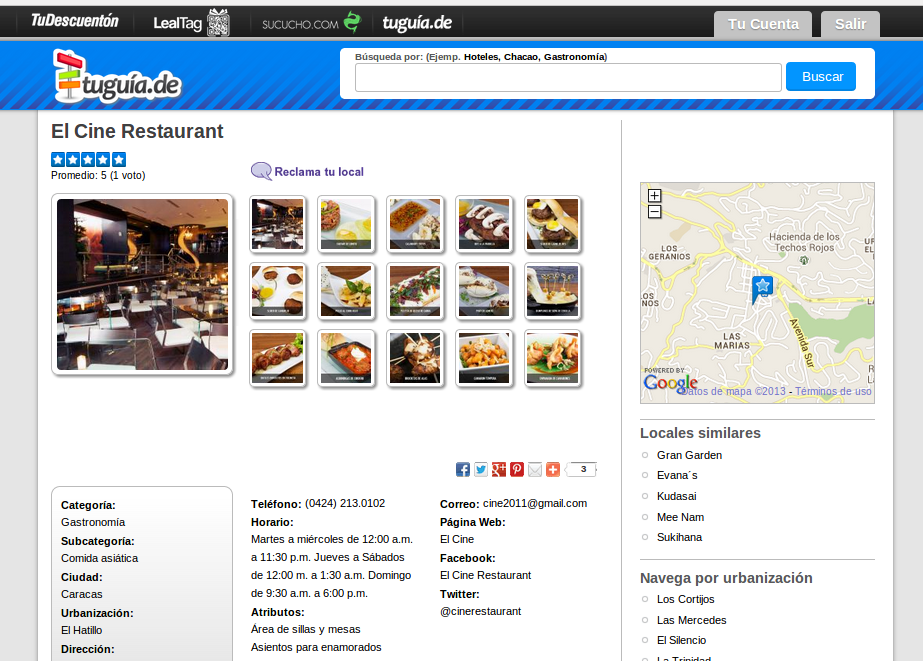
\includegraphics[scale=0.4]{imagenes/local_tgd.png}
	\end{center}
	\caption{
		\label{fig:localtgd}
		Local visto en \textit{Tuguia.de} 
	}
\end{figure}



\subsection{Taxonomías} \label{subsect:taxonomia}

Una taxonomía es un tipo de vocabulario o conjunto de palabras en que todos los términos están conectados, su objetivo es organizar la información y mejora la búsqueda de contenidos en los sitios web \cite{CM05}. En el caso de \textit{Tuguia.de} las taxonomías usadas son: 
\begin{itemize}
\item Ciudad.
\item Urbanización.
\item Categoría.
\item Subcategoría.
\item Atributos.
\end{itemize}

\subsection{Reseña} \label{subsect:resena}

"Para Tuguía.de, una reseña es un pequeño texto en donde el usuario cuenta su experiencia.  Puede ser también llamada "comentario". Éstas serán escritas en los cuadros de texto dentro de cada local, y servirán para que cada usuario cuente su historia"\cite{TGD}. Para que una reseña sea válida el usuario debe asignarle una calificación de uno a cinco al local que esta comentando.

 


